% ==================================================================
% INICIA PREÁMBULO DEL DOCUMENTO
% ==================================================================

% -----------DECLARACIÓN DE TIPO DE DOCUMENTO A DISEÑAR-------------

\documentclass[12pt]{uaztesis}

% % --------------DECLARACIÓN DE PAQUETES A UTILIZAR------------------

\usepackage[spanish,mexico]{babel}
\usepackage{subfigure}
\usepackage{multirow,rotating}
\usepackage[hidelinks]{hyperref}
\usepackage{graphicx}
\usepackage{float}
\usepackage{fancyhdr}
\usepackage{listings}
\usepackage{amssymb,amsmath,ams fonts}
\usepackage{tabularx,colortbl,xspace,rotating,booktabs,longtable,multirow}
\usepackage{soulutf8}
\usepackage{multirow} % para las tablas
\usepackage{longtable} % para tablas largas
\usepackage{multirow, array} % para las tablas
\usepackage{float} % para usar [H]
\usepackage{color,curves}
\usepackage{chngcntr}
\usepackage{minted}
\usepackage{csquotes}
\usepackage{pdfpages}

\renewcommand\listingscaption{C\'odigo}
\numberwithin{listing}{chapter}

% % --DECLARACIÓN DE RUTA DE CARPETA DONDE SE ENCUENTRAN LAS FIGURAS--
\graphicspath{{Imagenes/}}
\psfull

% % --------------DECLARACIÓN DEL ESTILO DE PÁGINA--------------------
\pagestyle{thesis}
\noappendixtables
\noappendixfigures

% % ===================================================================
% % INICIA EL CONTENIDO DEL DOCUMENTO
% % ===================================================================

\begin{document}

%\thesism % Tesis de maestria
\thesisd % Tesis de doctorado
%\thesis % Tesis licenciatura
%\degree{Ingeniero en Robótica y Mecatrónica} % Solo para licenciatura

% % Introducción en sílabas de palabras desconocidas por LaTeX
 \hyphenation{}

% % Declaración de número de páginas en números Romanos
 \clearpage\pagenumbering{roman}

% % ------------------INTRODUCCIÓN DE DATOS----------------------------

% % Título de la tesis, autor, y grado a recibir:
\title{Título de la tesis} 
\author{Estudiante}

% % Grado y nombre de asesores de tesis:
\advisortitle{Grado} \advisorname{Asesor} 
\gradosegundoasesor{Grado} \nombresegundoasesor{Asesor}
\gradotercerasesor{Grado} \nombretercerasesor{Asesor} % Si no hay tercer asesor, dejar en blanco

\date{\the\year{}}

% % ---------GENERACIÓN DE PÁGINAS PRELIMINARES DEL DOCUMENTO----------

% % Genera página de presentación
 \maketitle
% % Se incluyen los documentos de parte del posgrado

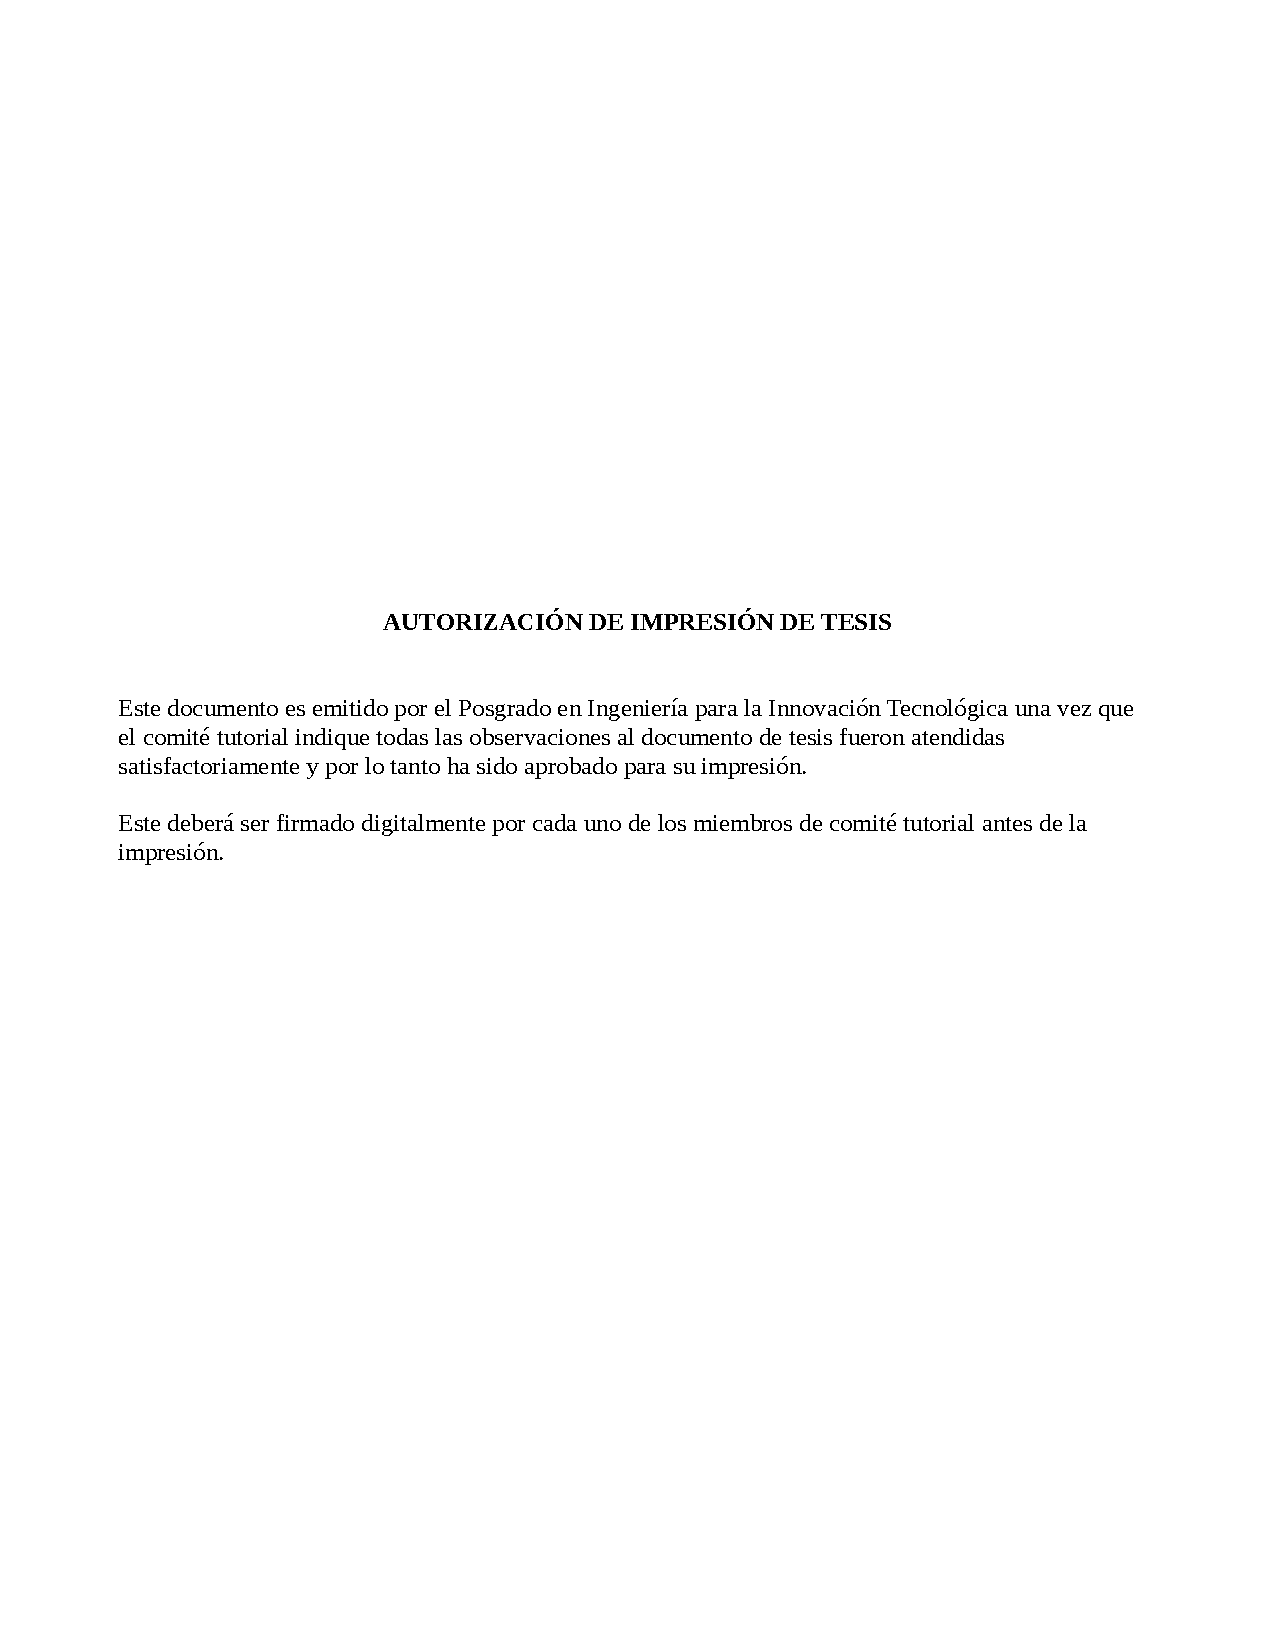
\includepdf[pages=-]{Adjuntos/autorizaciontesis.pdf}
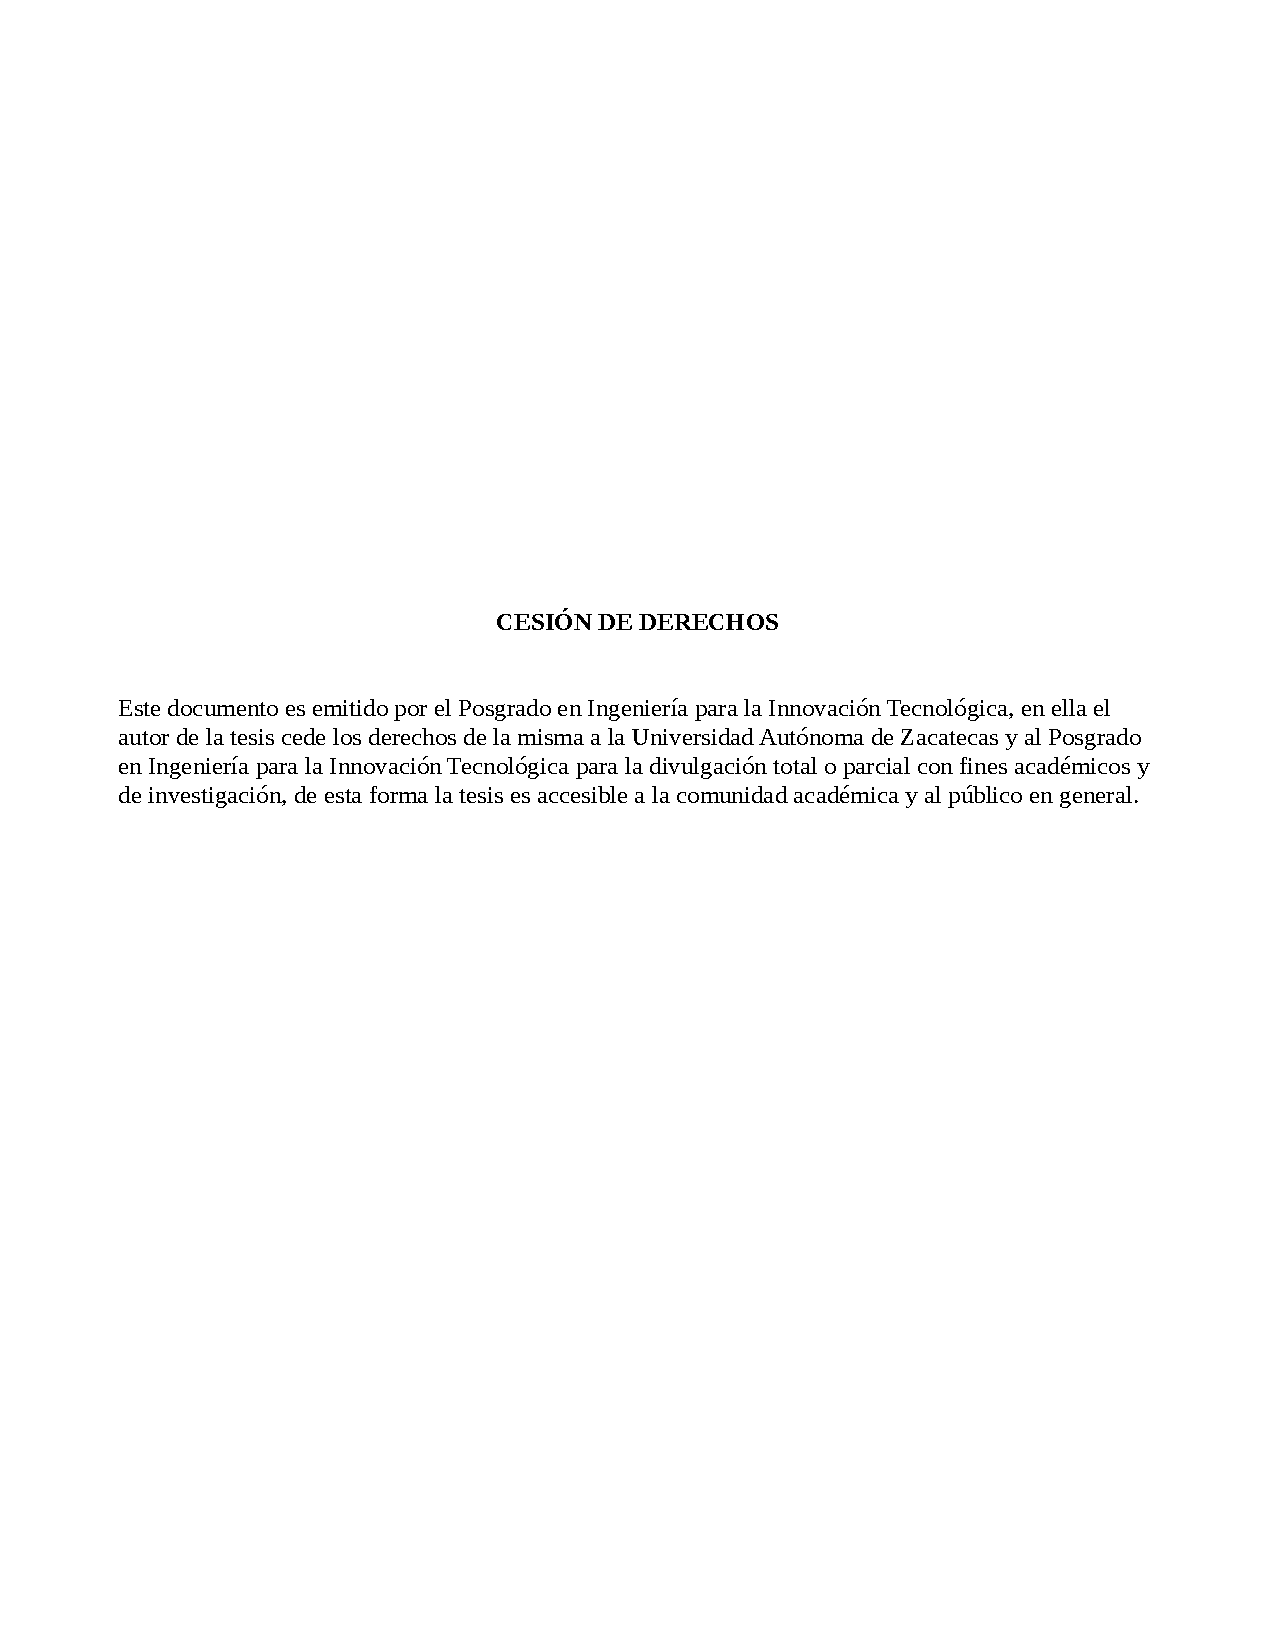
\includepdf[pages=-]{Adjuntos/cesionderechostesis.pdf}
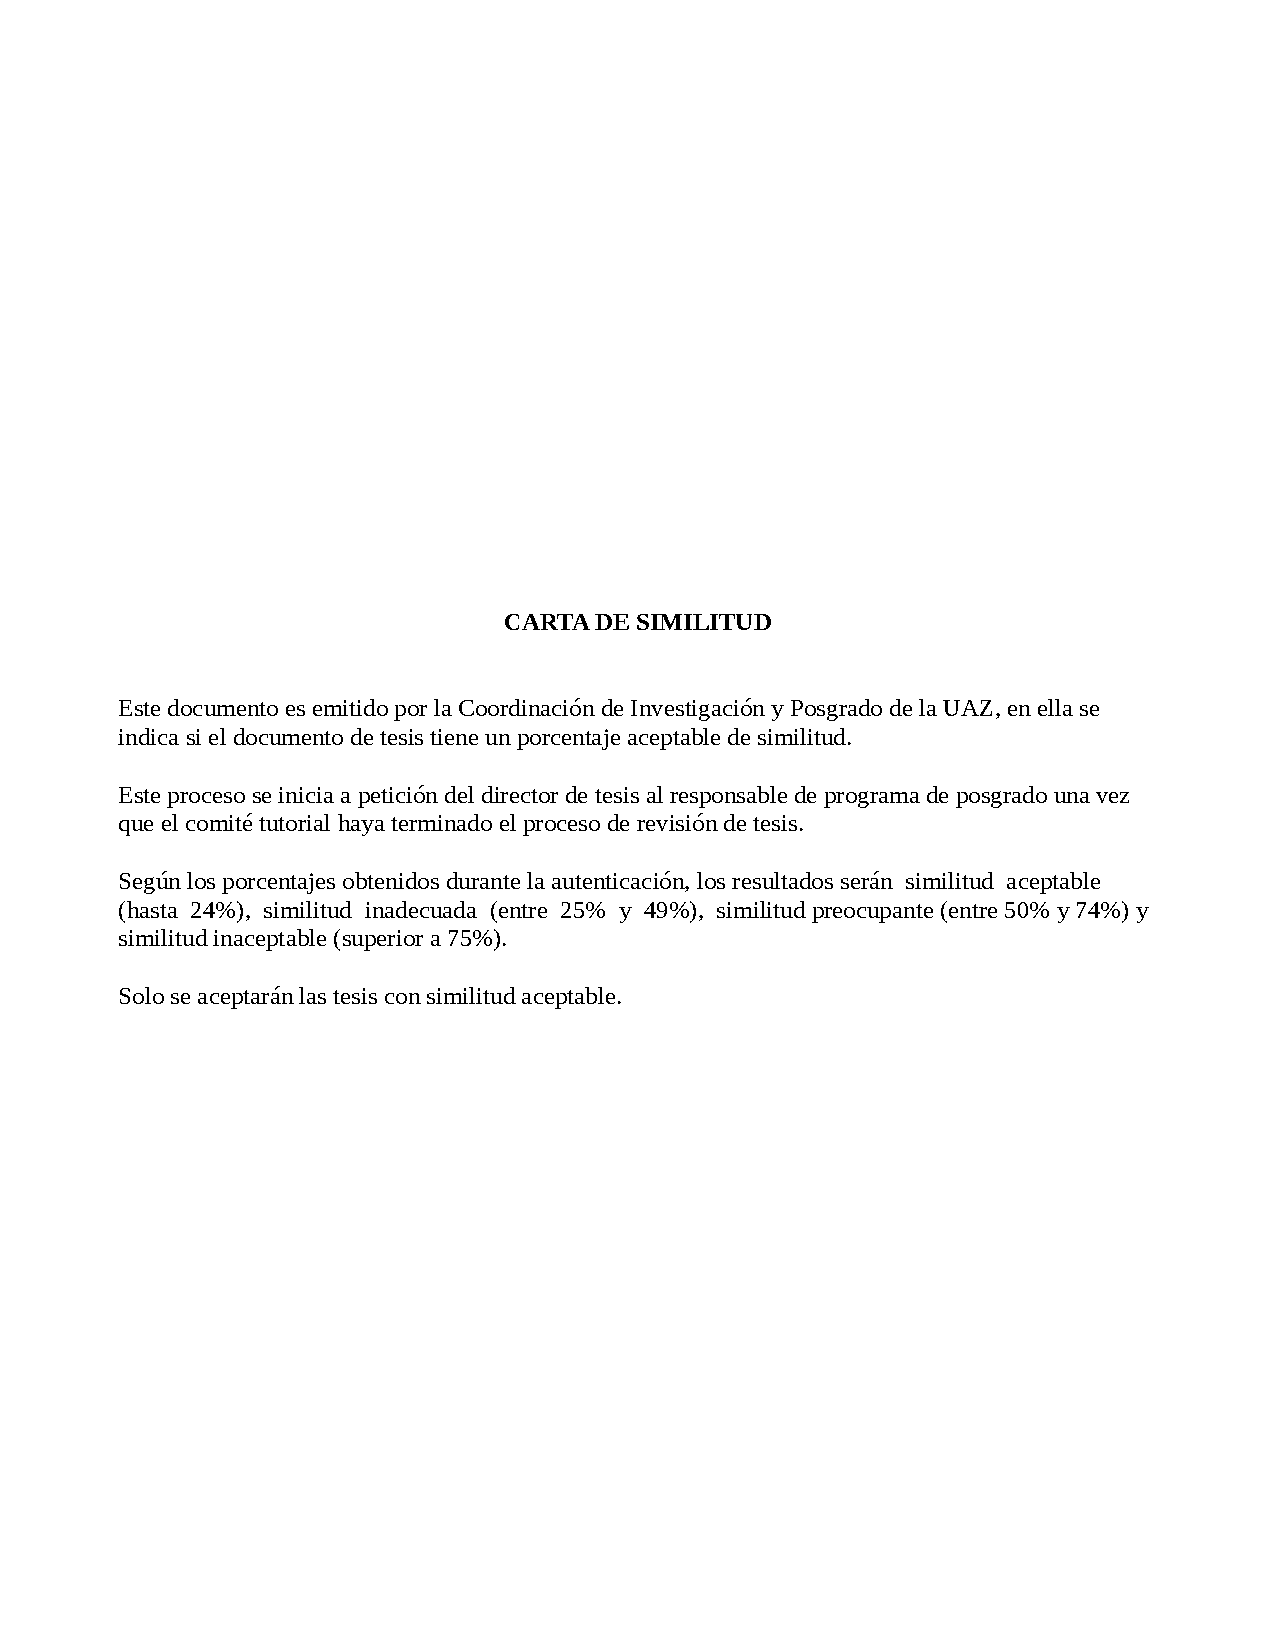
\includepdf[pages=-,scale=0.85]{Adjuntos/cartadesimilitud.pdf}

 % % Genera páginas de resumen
\begin{resumen}
  Esto es el resumen
          
\end{resumen}

\begin{abstract}
  The Abstract of a thesis is a brief yet comprehensive summary of the research, providing an overview of its objectives, methodology, key findings, and conclusions. It serves as a standalone section that allows readers to quickly grasp the essence of the study without having to read the entire document. A well-structured abstract ensures that the research is accessible and effectively communicates its significance.

In terms of structure, the abstract should include a brief introduction to the research problem, followed by the main objectives or research questions. It should then summarize the methodology used, highlighting the key techniques and approaches. The abstract must also present the most important results and conclude with the main implications or contributions of the study. It should be written in a concise, objective, and impersonal style, avoiding citations, figures, or tables.

Regarding length, the abstract for a Master's thesis should not exceed 350 words, while for a Doctoral dissertation, it can be up to 500 words. It is important to ensure that the abstract is self-contained, meaning that it provides sufficient information for the reader to understand the research without additional context.          
\end{abstract}

% % Genera página de dedicatoria
\begin{dedicatoria}
  En esta sección se puede expresar su gratitud y reconocimiento a personas o entidades que han influido positivamente en su vida académica, profesional o personal, y que han brindado apoyo durante el proceso de investigación y redacción de la tesis. 

Es una parte personal y emotiva del documento, que permite al autor reconocer y honrar a quienes contribuyeron a su éxito y esfuerzo académico. Esta debe ser corta, en una sola página.          
\end{dedicatoria}

 % Genera página de agradecimientos
\begin{agradecimientos}
  En esta sección se expresa su gratitud y reconocimiento a todas las personas e instituciones que han contribuido directa o indirectamente al desarrollo y culminación de su trabajo de investigación. Esta sección es una oportunidad para mostrar aprecio por el apoyo, la orientación y los recursos proporcionados durante el proceso de elaboración de la tesis.

La estructura es la siguiente:

\begin{enumerate}
    \item Al director de tesis
    \item A familiares y amigos
    \item A los compañeros de investigación
    \item Al Posgrado en Ingeniería para la Innovación Tecnológica y docentes
    \item A la Universidad Autónoma de Zacatecas
    \item Al CONAHCYT (en caso de ser becario)
\end{enumerate}

Un ejemplo de agradecimiento al CONAHCYT es: Al Sistema Nacional de Posgrados (SNP) del Consejo Nacional de Humanidades, Ciencia y Tecnología (CONAHCYT) por su apoyo económico a través de la convocatoria "Becas Nacionales (Tradicional) 20xx-20xx".        
\end{agradecimientos}

% % Genera páginas del contenido general y lista de figuras y tablas
\tableofcontents
\listoffigures                 
\listoftables                  

\begin{nomenclatura}
    \begin{description}
\item{\makebox[2.5cm][l]{$cd$}} Corriente directa.
\item{\makebox[2.5cm][l]{$ca$}} Corriente alterna.
\item{\makebox[2.5cm][l]{$NdFeB$}} Neudimio-Fierro-Boro.
\item{\makebox[2.5cm][l]{$FEM$}} Fuerza electromotriz.
\item{\makebox[2.5cm][l]{$FMM$}} Fuerza magnetomotriz.
\end{description}
\end{nomenclatura}

\begin{listofsymbols}
    \begin{description}
\item{\makebox[1.2cm][l]{$\mu_0$} \makebox[2.2cm][l] {$[Wb/A \cdot m]$}} Permeabilidad magnética del espacio libre.
\item{\makebox[1.2cm][l]{$\mu_{rFe}$} \makebox[2.2cm][l] { }} Permeabilidad magnética relativa del acero.
\item{\makebox[1.2cm][l]{$\rho$} \makebox[2.2cm][l] {$[kg/m^{3}]$}} Densidad de masa del aire.
\item{\makebox[1.2cm][l]{$\rho_{cu}$} \makebox[2.2cm][l] {$[kg/m^{3}]$}} Densidad de masa del cobre.
\item{\makebox[1.2cm][l]{$H$} \makebox[2.2cm][l] {$[A/m]$}} Intensidad de campo magnético.
\item{\makebox[1.2cm][l]{$\phi_r$} \makebox[2.2cm][l] {$[Wb]$}}  Flujo magnético remanente.
\item{\makebox[1.2cm][l]{$\eta$} \makebox[2.2cm][l] { }} Eficiencia.
\item{\makebox[1.2cm][l]{$\lambda$} \makebox[2.2cm][l] { }} Velocidad específica o TSR.
\item{\makebox[1.2cm][l]{$T$} \makebox[2.2cm][l] {$[N \cdot m]$}} Par o torque.
\item{\makebox[1.2cm][l]{$I$} \makebox[2.2cm][l] {$[A]$}} Corriente eléctrica.
\item{\makebox[1.2cm][l]{$R$} \makebox[2.2cm][l] {$[\Omega]$}} Resistencia eléctrica.
\end{description}
\end{listofsymbols}

\begin{glosario}
   \input{07_Glosario}
\end{glosario}

% %--------INCLUSIÓN DE LOS ARCHIVOS (CAPÍTULOS) DEL DOCUMENTO--------

% % Declaración de número de páginas en números Arábigos
 \clearpage\pagenumbering{arabic}

% incluye los captitulos de la tesis
\chapter{Introducción}

\section{Planteamiento del problema}

\section{Hipótesis}


\section{Justificación}


\section{Objetivos}

\subsection{Objetivo general}

\subsection{Objetivos particulares}

\section{Alcances y limitaciones}

\section{Metodología}
 








  






\chapter{Marco Teórico}

El marco teórico es una sección fundamental que proporciona la base conceptual y teórica sobre la cual se sustenta la investigación. En esta sección, se revisan y analizan las teorías, conceptos, estudios previos y trabajos relevantes que están directamente relacionados con el problema de investigación. El propósito del marco teórico es situar la investigación dentro del contexto académico y científico existente, y justificar el enfoque y los métodos seleccionados.

El marco teórico  debe proporcionar una base sólida y bien fundamentada que respalde la investigación. Al revisar la literatura existente, describir teorías y conceptos clave, y justificar el enfoque metodológico, este marco ayuda a situar la investigación dentro del contexto académico y científico adecuado.

Los componentes del Marco Teórico son:

\begin{enumerate}
    \item Introducción del Marco Teórico:
    \begin{enumerate}
        \item Breve introducción que explique el propósito del marco teórico y su relevancia para la investigación.
        \item Descripción del enfoque general y la estructura del marco teórico.
    \end{enumerate}
    \item Revisión de la Literatura:
    \begin{enumerate}
        \item Antecedentes Históricos: Contexto histórico del tema de estudio, incluyendo el desarrollo y la evolución de las teorías relevantes.
        \item Estudios Previos: Resumen y análisis de investigaciones previas relacionadas con el problema de investigación. Se destacan los hallazgos clave, metodologías utilizadas y brechas identificadas en el conocimiento.
        \item Estado del Arte: Exposición de las tecnologías, métodos y avances más recientes en el área de estudio. Esto puede incluir una revisión de las innovaciones tecnológicas, nuevas metodologías o enfoques teóricos.
    \end{enumerate}
    \item Teorías y Conceptos Relevantes:
    \begin{enumerate}
        \item Teorías Fundamentales: Descripción detallada de las teorías y modelos teóricos que forman la base de la investigación. Se debe explicar cómo estas teorías se aplican al problema de estudio.
        \item Conceptos Clave: Definición y explicación de los conceptos fundamentales utilizados en la investigación. Esto puede incluir términos técnicos, principios de ingeniería y conceptos científicos.
    \end{enumerate}
    \item Modelos y Enfoques Metodológicos:
    \begin{enumerate}
        \item Modelos Matemáticos y Computacionales: Presentación de los modelos teóricos y computacionales que serán utilizados o desarrollados en la investigación. Se deben explicar las ecuaciones y su relevancia.
        \item Metodologías de Investigación: Descripción de las metodologías y técnicas empleadas en estudios anteriores que son relevantes para el enfoque de la investigación actual.
    \end{enumerate}
    \item Relación del Marco Teórico con la Investigación:
    \begin{enumerate}
        \item Justificación del Enfoque: Explicación de cómo las teorías y conceptos revisados justifican y apoyan el enfoque metodológico elegido para la investigación.
        \item Integración de la Literatura: Síntesis de cómo los estudios previos, teorías y conceptos se integran para formar el marco conceptual de la investigación.
    \end{enumerate}
    \item Identificación de Brechas y Oportunidades:
    \begin{enumerate}
        \item Brechas en el Conocimiento: Identificación de las áreas que no han sido suficientemente exploradas o que presentan controversias en la literatura existente.
        \item Oportunidades de Investigación: Presentación de las oportunidades que estas brechas ofrecen para el desarrollo de nuevas investigaciones y contribuciones al campo de estudio.
    \end{enumerate}
\end{enumerate}
\chapter{Desarrollo}

\textbf{Cómo citar utilizando BibLaTeX}

BibLaTeX es una herramienta  para gestionar y generar referencias en documentos escritos con LaTeX. Ofrece una variedad de comandos para citar fuentes de manera adecuada según el contexto.

A continuación, se describe cómo usar los principales comandos para citar y se incluyen ejemplos prácticos.

\textbf{Comandos principales para citar}

\begin{enumerate}
    \item \textbackslash cite
    Este comando genera una cita compacta que usualmente incluye solo el autor y el año, o un número si se utiliza un estilo numérico.

    Uso típico: Se emplea en notas al pie o en listados donde no es necesario integrar la cita en el texto.
    
    Ejemplo:
    
    
    Según los resultados presentados en varios estudios \textbackslash cite\{smith2010data\}, el modelo es efectivo.
    
    Según los resultados presentados en varios estudios \cite{smith2010data}, el modelo es efectivo.
    
    \item \textbackslash parencite

    Genera una cita entre paréntesis que incluye el autor y el año o el identificador correspondiente al estilo elegido.
    Uso típico: Ideal para citas parentéticas en texto fluido.

    Ejemplo:

    El rendimiento de los sistemas GNSS ha sido evaluado (véase \textbackslash parencite\{johnson2015gps\}).


    El rendimiento de los sistemas GNSS ha sido evaluado (véase \parencite{johnson2015gps}).

    \item \textbackslash textcite

    Integra la referencia directamente en el flujo del texto, mencionando explícitamente el nombre del autor y el año.
    Uso típico: Perfecto para dar énfasis a los autores en el cuerpo del texto.

    Ejemplo:

    \textbackslash textcite\{doe2018antenna\} destacan que las antenas log-periódicas son altamente efectivas para aplicaciones de radar.

    \textcite{doe2018antenna} destacan que las antenas log-periódicas son altamente efectivas para aplicaciones de radar.

\end{enumerate}

\textbf{Ejemplo práctico de uso en un documento}

El desarrollo de antenas para aplicaciones de radar ha sido un tema de amplio interés. \textbackslash textcite\{smith2010data\} propusieron un diseño optimizado para frecuencias de microondas. Otros estudios, como los de \textbackslash parencite\{johnson2015gps\}, se han enfocado en la integración con sistemas GNSS.

Un análisis comparativo demuestra que \textbackslash cite\{doe2018antenna\} lograron mejores resultados al implementar estructuras log-periódicas.


El desarrollo de antenas para aplicaciones de radar ha sido un tema de amplio interés. \textcite{smith2010data} propusieron un diseño optimizado para frecuencias de microondas. Otros estudios, como los de \parencite{johnson2015gps}, se han enfocado en la integración con sistemas GNSS.

Un análisis comparativo demuestra que \cite{doe2018antenna} lograron mejores resultados al implementar estructuras log-periódicas.

\textbf{Citas con varias fuentes}

Cuando necesitas citar varias fuentes al mismo tiempo con BibLaTeX, puedes incluir múltiples claves de entrada en el mismo comando de citación, separadas por comas. Esto se aplica a los comandos como \textbackslash cite, \textbackslash parencite y \textbackslash textcite. A continuación, se muestra cómo hacerlo con ejemplos prácticos.

Ejemplo de citar varios autores al mismo tiempo

\begin{enumerate}
    \item Con \textbackslash cite

    Genera una cita compacta con todas las fuentes mencionadas.
    
    Diversos estudios han analizado el impacto de las antenas log-periódicas en aplicaciones de radar \textbackslash cite\{smith2010data, johnson2015gps, doe2018antenna\}.

    Diversos estudios han analizado el impacto de las antenas log-periódicas en aplicaciones de radar \cite{smith2010data, johnson2015gps, doe2018antenna}.

    \item Con \textbackslash parencite

    Incluye la lista de citas en un formato parentético.
    
    El rendimiento del sistema ha sido evaluado previamente (véase \textbackslash parencite\{smith2010data, johnson2015gps, doe2018antenna\}).

    El rendimiento del sistema ha sido evaluado previamente (véase \parencite{smith2010data, johnson2015gps, doe2018antenna}).

    \item Con \textbackslash textcite

    Integra varios autores en el texto.
    
    Trabajos recientes como los de \textbackslash textcite\{smith2010data\}, \textbackslash textcite\{johnson2015gps\} y \textbackslash textcite\{doe2018antenna\} han destacado diferentes aspectos del diseño y rendimiento de estas tecnologías.

    Trabajos recientes como los de \textcite{smith2010data}, \textcite{johnson2015gps} y \textcite{doe2018antenna} han destacado diferentes aspectos del diseño y rendimiento de estas tecnologías.
    
\end{enumerate}

\textbf{Resumen de recomendaciones para citar}

\begin{enumerate}
    \item \textbackslash cite: Úsalo para citas generales o en listados compactos.
    \item \textbackslash parencite: Utilízalo cuando necesites incluir la cita entre paréntesis.
    \item \textbackslash textcite: Prefiérelo para integrar la referencia de forma fluida en el texto.
\end{enumerate}

El archivo Referencias.bib es donde se almacenan las entradas bibliográficas.

Esta flexibilidad te permite adaptar tus citas al estilo de redacción que prefieras, manteniendo un formato académico correcto.
\chapter{Resultados}








\chapter{Conclusiones}



% % ------------------INTRODUCCIÓN DE REFERENCIAS---------------------

\nocite{*}
\chapter*{Referencias bibliográficas}     
\addcontentsline{toc}{chapter}{Referencias bibliográficas}
\printbibliography[heading=none]

% % ---------------------INTRODUCCIÓN DE APÉNDICES--------------------

\begin{apendices}
\chapter{Título}
\chapter{Título}


\end{apendices}


\end{document}